\documentclass{beamer}

% Theme and color scheme
\usetheme{Madrid}
\usecolortheme{whale}
\usepackage{xcolor}
\usepackage{etoolbox}

% Packages
\usepackage{graphicx}
\usepackage{hyperref}
\usepackage[backend=biber, sorting=none]{biblatex}
\addbibresource{refs.bib}
\DeclareFieldFormat*{title}{#1}
\DeclareFieldFormat*{url}{\newline\url{#1}\nopunct}
\DeclareFieldFormat{labelnumberwidth}{#1\adddot}
\setlength{\biblabelsep}{5pt}
\renewcommand*{\bibfont}{\tiny}
\usepackage{ragged2e}

\newcommand{\biburl}[2][]{%
  \newline - \ifstrempty{#1}{}{\textcolor{cyan}{#1: }}\url{#2}\nopunct
}

\title{ChatGPT Survey}
\subtitle{A Programmer's Perspective}
\author{Yu Zehan}
\institute{Intel FLEX}
\date{\today}

\begin{document}

\begin{frame}
  \titlepage
\end{frame}

\begin{frame}{Outline}
  \tableofcontents
\end{frame}

\section{Before Coding}
\begin{frame}{Before Coding}
    \begin{itemize}
        \item Planning and Analysis
        \begin{itemize}
            \item Defining Project Goals and Requirements
            \item Analyzing Feasibility of Proposed Solutions
            \item Creating User Stories and Acceptance Criteria
        \end{itemize}
        \item Design
        \begin{itemize}
            \item Designing System Architecture and Components
            \item Creating Wireframes and Mockups of User Interface
            \item Designing Database Schema and Defining APIs
        \end{itemize}
        \item Tool Selection and Setup
        \begin{itemize}
            \item Selecting Development Tools and Technologies
            \item Setting up Development Environment
            \item Configuring Version Control and Collaboration Tools
        \end{itemize}
    \end{itemize}
\end{frame}

\section{During Coding}
\subsection{Implementation}
\begin{frame}{Implementation}
    \begin{itemize}
        \item Writing Business Logic and Implementing User Interface
        \item Integrating with External Systems and APIs
        \item Setting up Data Storage and Retrieval
    \end{itemize}
\end{frame}

\begin{frame}{Testing and Debugging}
  \begin{itemize}
      \item Writing Automated Tests for Each Component of System
      \item Performing Functional, Integration, and System Testing
      \item Debugging and Fixing Errors in Code
  \end{itemize}
\end{frame}

\subsection{Deployment}
\begin{frame}{Deployment}
  \begin{itemize}
      \item Setting up Continuous Integration and Deployment Pipelines
      \item Deploying System to Production Environment
      \item Monitoring System Performance and Stability
  \end{itemize}
\end{frame}

\section{After Coding}
\begin{frame}{After Coding}
  \begin{itemize}
      \item Maintenance
      \begin{itemize}
          \item Fixing Bugs and Implementing New Features
          \item Updating Dependencies and Patching Security Vulnerabilities
          \item Monitoring System Performance and Stability
      \end{itemize}
      \item Refactoring and Optimization
      \begin{itemize}
          \item Identifying Opportunities for Code Refactoring
          \item Improving Code Readability and Maintainability
          \item Optimizing System Performance and Resource Usage
      \end{itemize}
      \item Documentation and Knowledge Transfer
      \begin{itemize}
          \item Updating System Documentation
          \item Writing Technical Reports and Presentations
          \item Training New Team Members and Transferring Knowledge
      \end{itemize}
  \end{itemize}
\end{frame}

\section{Iterative Coding}
\begin{frame}{Iterative Coding}
    \begin{itemize}
        \item Iterative Development Process
        \begin{itemize}
          \item Planning and Prioritizing Features for Each Iteration
          \item Implementing Features and Testing in Each Iteration
          \item Reviewing and Demonstrating Features to Stakeholders
      \end{itemize}
      \item Continuous Integration and Delivery
      \begin{itemize}
          \item Integrating Code Changes and Running Automated Tests
          \item Deploying Changes to Staging and Production Environments
          \item Monitoring System Performance and Stability
      \end{itemize}
      \item Feedback and Improvement
      \begin{itemize}
          \item Gathering Feedback from Stakeholders and Users
          \item Analyzing Feedback and Identifying Areas for Improvement
          \item Implementing Improvements and Refining Development Process
      \end{itemize}
  \end{itemize}
\end{frame}

\begin{frame}{TikZ Test}
  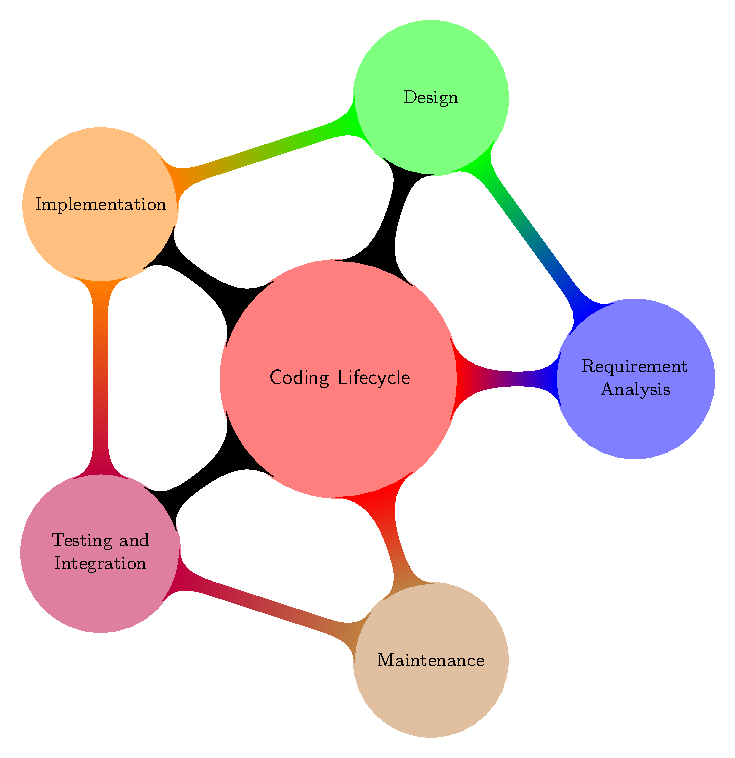
\includegraphics[width=\textwidth,height=0.8\textheight,keepaspectratio]{tikz-code-lifecycle.pdf}
\end{frame}



% 行动指南(instructions)、事实依据(facts)、思想纲领(policies)

\section{References}
\begin{frame}[t,allowframebreaks]{References}
  \nocite{*}
  \RaggedRight
  \printbibliography
\end{frame}


% Closing slide
\begin{frame}{FAQ}

\end{frame}

\end{document}
